\documentclass[a4paper, 11pt]{article}
\usepackage{comment} % enables the use of multi-line comments (\ifx \fi) 
\usepackage{fullpage} % changes the margin
\usepackage{graphicx}
\usepackage{amsmath}

\begin{document}
\thispagestyle{empty}
%Header-Make sure you update this information!!!!
\noindent
\large\textbf{AmBe Detector Calibration Calculations} \\
\hfill John Boyington \\
\hfill Kansas State University \\

\vspace{0.03\textheight}

%%%%%%%%%%%%%%%%%%%%%%%%%%%%%%%%%%%%%%%%%%%%%%%%%%%%%%%%%%%%%%%%%%%%
%                           SUMMARY
%%%%%%%%%%%%%%%%%%%%%%%%%%%%%%%%%%%%%%%%%%%%%%%%%%%%%%%%%%%%%%%%%%%%

The document describes the calculations used to obtain the absolute efficiency of the LiI neutron detector used in Bonner Sphere measurements.

\section{Source Term}

The following equation was used to determine $W$, a value for the {\tt WGT} parameter on the source SDEF card, which represents the total number of source neutrons emitted during the measurement period.

$$ W = A t 3.7 \times 10^{10} \textrm{(Bq/Ci)} $$

Here, $A$ is the source activity, 4.85 Ci, $t$ is the total measurement time, 60s, and $3.7 \times 10^{10}$ is the conversion from Ci to Bq. This equation yields a value of $1.0767 \times 10^{13}$ for $W$. Below is given a PDF of the energy-dependent source spectrum.


\begin{figure}[hb]

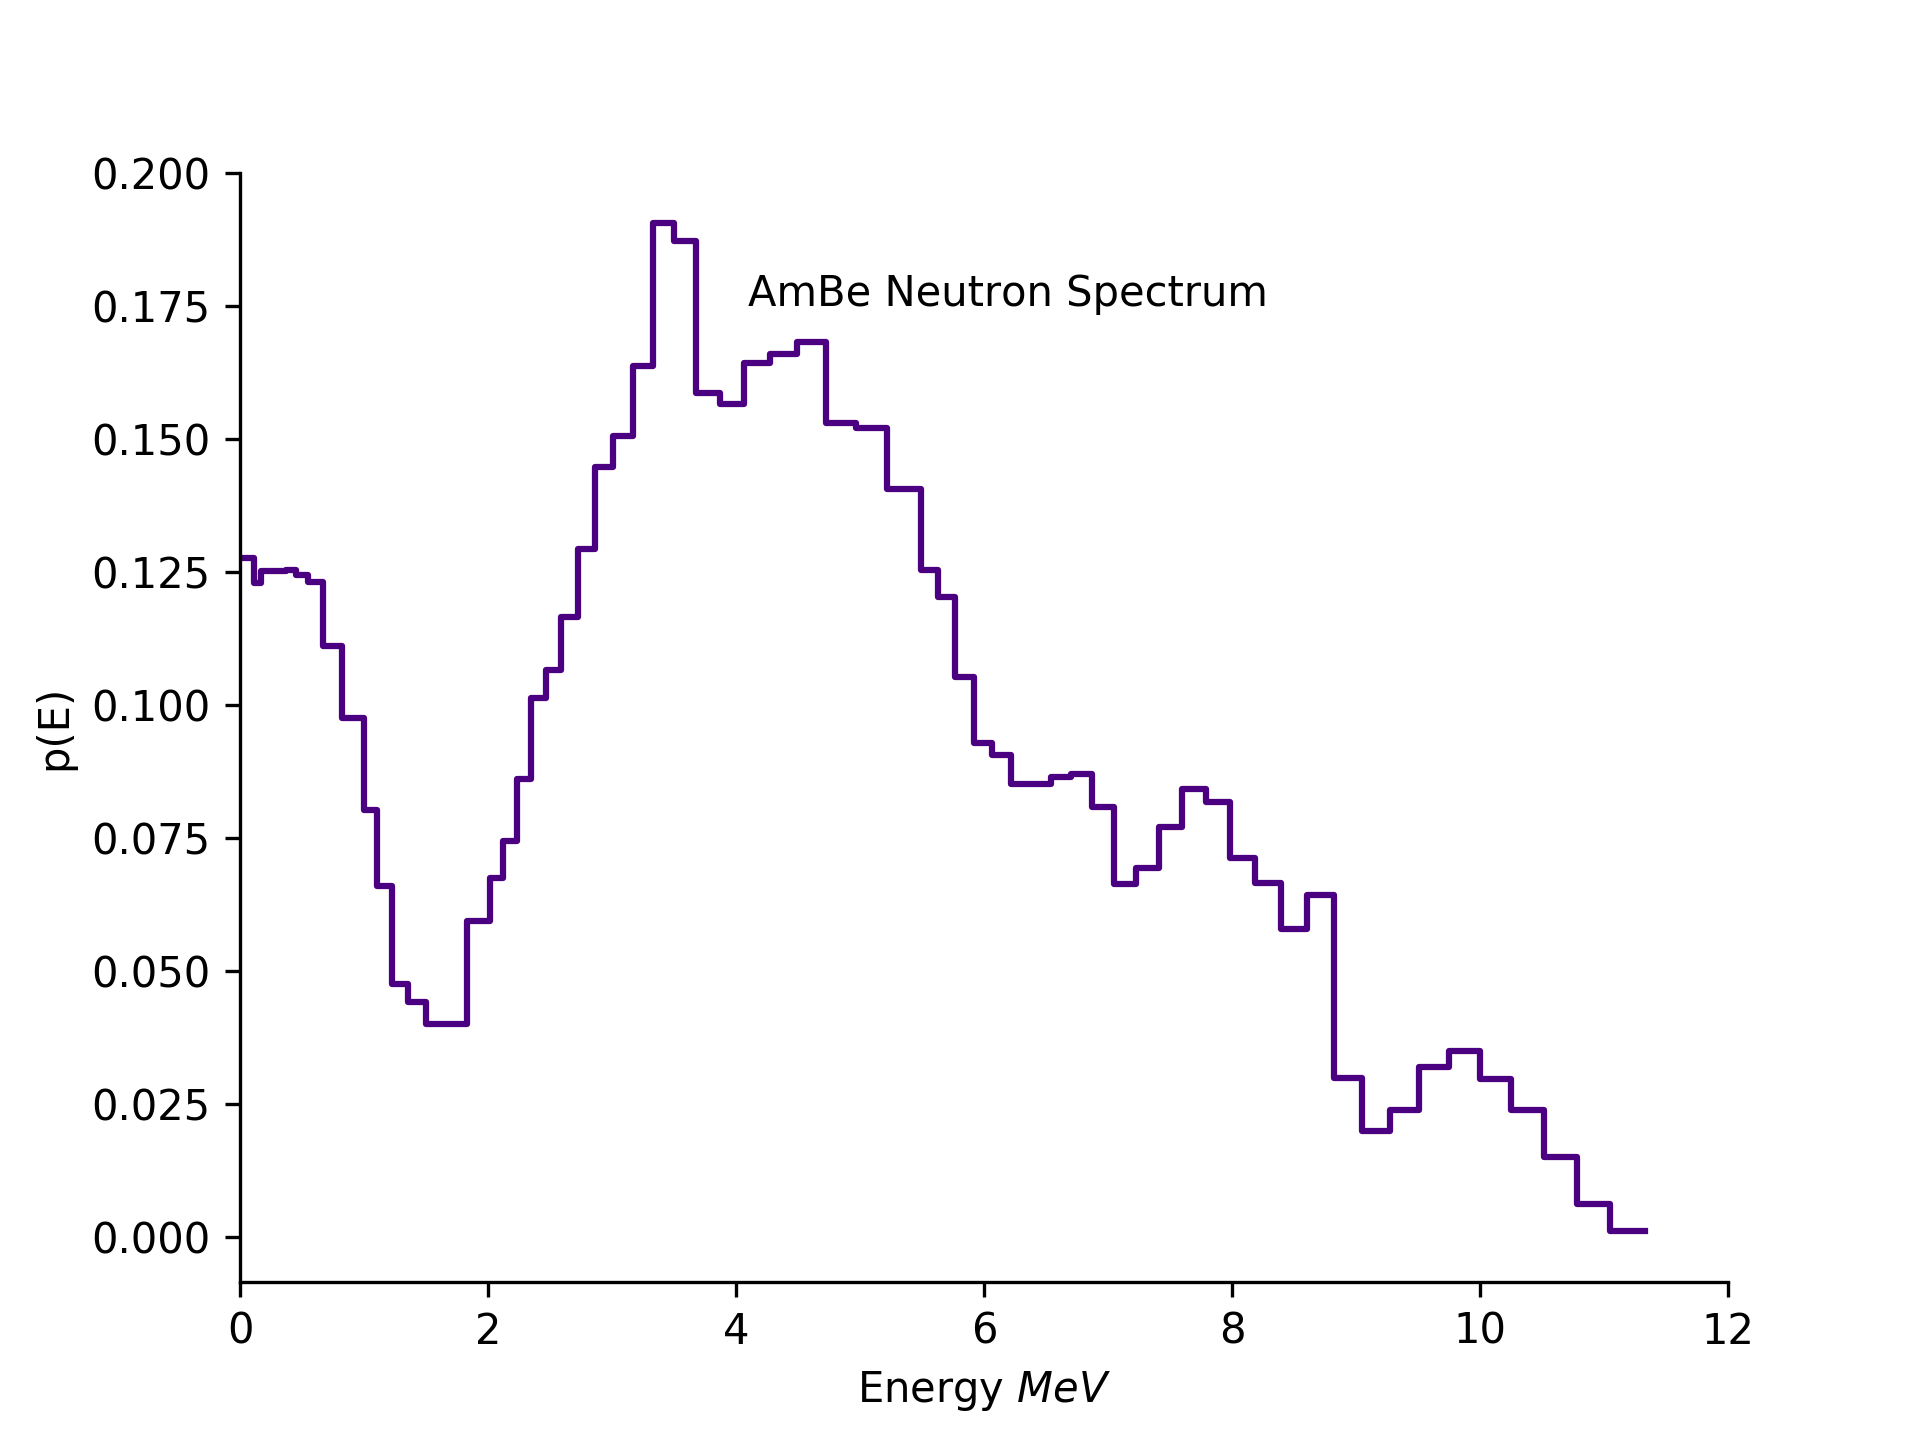
\includegraphics[]{ambe_bare}
\end{figure}

\section{Tally Normalization}

The result of the MCNP F4 tally will be given in units of [1/cm$^2$]. By using a tally multiplier card with an ENDF reaction number of 105, that value will be multiplied by the microscopic cross section $\sigma$[barns]. A constant of proportionality, $C$, equal to the atomic number density $N$ in [1/b $\cdot$ cm] times the volume $V$ in [cm$^3$] is needed to convert this fluence value into a total reaction rate.

$$ R = C \int \Phi(E) \sigma(E) dE $$

where

$$ C = V N \frac{1}{10^{24}} \textrm{(barns/cm$^2$)} $$

and

$$ N = \frac{\rho N_A}{M} $$

In this case, $N$ is reported as $1.74 \times 10^{22}$ [atoms/cm$^3$] in a paper by Decker. The detector volume $V$ is a 4mm $\times$ 4mm cylinder, and therefore equal to $\pi (\frac{D}{2})^2 h$, or 0.0502645 cm$^3$. The value for $C$ calculated using these parameters is thus 8.7965 $\times 10^{-4}$ cm$^2$/barn.

\section{Efficiency Calculation}

Experimentally, for a 60s count, a total experimental response, $R_e$, of 53,016 counts were measured (53,161 gross cpm - 145 background cpm). The MCNP result for the response was found to be 580,541. The following equation is used to determine the detection efficiency of the detector.

$$ \textrm{efficiency} = \frac{R_{e}}{R_{mc}} $$

Therefore, the overall efficiency of the detector is:

$$ \textrm{efficiency} = 0.0913 $$

\end{document}

